% \documentclass[a4paper,10pt]{article}
 \documentclass[review,times,3p,twocolumn,10pt]{elsarticle}
\usepackage[utf8]{inputenc}

\usepackage{graphicx}
\usepackage{graphics}
\usepackage{enumitem}

\usepackage{epsfig}
\usepackage{subfigure}
\usepackage{tabularx}
\usepackage{amssymb}
\usepackage{amsmath}

\usepackage{colortbl}

\usepackage{enumitem}
% \usepackage{a4wide} %full page
\usepackage{fullpage}
\usepackage{hyperref}
\usepackage{natbib}
\usepackage{amsmath,amssymb}
\usepackage{setspace}
\usepackage[scientific-notation=true]{siunitx} %VVV
\sisetup{round-mode = places, round-precision = 3} %VVV
\doublespacing

\usepackage{booktabs}
\usepackage{multirow}
\usepackage{url}

%  \usepackage{multirow}
 \usepackage[table,xcdraw]{xcolor}

% \usepackage{jabbrv}

\usepackage{blindtext}
\usepackage{todonotes}

 \RequirePackage{lineno} 

\bibliographystyle{model2-names}
\biboptions{authoryear}

\newenvironment{lineq}
    {\begin{linenomath*}
    \begin{equation}
    }
    { 
    \end{equation} 
    \end{linenomath*}
    }


\newcommand{\dd}{\mathrm{d}}
\renewcommand{\vec}{\mathbf}
 \newcommand{\subscript}[2]{$#1 _ #2$}

 \newcommand{\Lb}{\pazocal{L}}
 
\newcommand{\fs}{\footnotesize}
    \renewcommand{\arraystretch}{1.5}



\journal{Advances in Water Resources}

\begin{document}

\begin{frontmatter}

\title{Issues in the inverse modeling of a single ring infiltration experiment}

\author[autor1]{Michal Kuraz}

\author[autor1]{Lukas Jacka}

\author[autor1]{Johanna Ruth Bloecher}

\author[autor2]{Matej Leps}



\address[autor1]{Czech University of Life Sciences Prague, Faculty of Environmental Sciences, Department of Water Resources and Environmental Modeling}

\address[autor2]{Czech Technical University in Prague, Faculty of Civil Engineering, Department of Mechanics}

\begin{abstract}
This contribution addresses issues in the identification of soil hydraulic properties (SHP) of the top soil layer obtained from inverse modeling of a single ring (SR) infiltration experiment. 
The SR experimental data were obtained from a series of in situ experiments conducted on a highly heterogeneous mountainous podzolic soil profile. The SHP of the topsoil layer are very difficult to measure directly, since the thickness of the top soil layer is often much smaller than the depth required to embed the SR or Guelph permeameter device or to obtain undisturbed samples for further laboratory experiments.

A common problem with automatic optimization procedures are convergence issues. This problem is not trivial and can be difficult to deal with. We present a methodology to avoid convergence issues with the nonlinear operator. With this methodology, we can answer (1) to what extent the well-known SR experiment is robust enough to provide a unique estimate of SHP parameters using the unsteady part of the infiltration experiment and (2) whether all parameters are vulnerable to non-uniqueness. We validated our methodology with synthetic infiltration benchmark problems for clay and sand. To evaluate non-uniqueness, local optima were identified and mapped using a modified genetic algorithm with niching, which is not possible with commonly used gradient methods. 

Our results show the existence of multimodality in, both, the benchmark problems and the real-world problem. This is an important finding as local optima can be identified, which are not necessarily physical and also for systems that do not exhibit multimodal grain size distributions. The identified local optima were distinct and showed different retention and hydraulic conductivity curves. The most physical set of SHP could be identified with the knowledge of saturated water content, which makes it yet more obvious that expert knowledge is key in inverse modeling.   


%To evaluate non-uniqueness, local optima were identified and mapped using a modified genetic algorithm with niching.   
%We also discuss important issues regarding (i) the design of the numerical simulations and (ii) the influence of spatial and temporal discretization on the identified local optima.

\end{abstract}

\begin{keyword}
soil hydraulic properties \sep inverse modeling \sep Richards equation \sep convergence issues  \sep automatic calibration \sep computational issues in geosciences  

%% MSC codes here, in the form: \MSC code \sep code
%% or \MSC[2008] code \sep code (2000 is the default)

\end{keyword}

\end{frontmatter}

\linenumbers

\section{Introduction}%[lukas]
% -motivace

Soil hydraulic properties (hereafter SHP) are important for many hydrological models and engineering applications. The mountainous podzolic soil evaluated here is typical for the source areas of many major rivers in the Central European region. The top layer of the soil plays a key role in the rainfall-runoff process, because it is the top-soil that separates the rainfall into surface runoff and subsurface runoff. 


Due to the rocks present and the dense root system of the covering vegetation, and due to the possible extension of the representative elementary volume, it is often impossible to collect undisturbed samples of top-soil for laboratory measurements in order to obtain the SHP parameters~\citep{Jacka1}. The SHP of the topsoil are therefore very difficult to measure directly~\citep{Fodor, Jacka1}. 


In our study, the well-known single ring (hereafter SR) method was used to obtain experimental input data (cumulative infiltration) for inverse modeling. The SR infiltrometer is a widely accepted, simple, robust field method, which is able to measure the infiltration process, which affects the entire soil profile including the top-soil,  and can sample a relatively large volume (depending on the diameter of the ring)~\citep{Cheng,ReynoldsWD}.  The SR infiltration experiment is an in situ experiment, which does not require soil samples to be collected, so the porous medium is kept relatively undisturbed. With the widely-used ring diameter of 30~cm, the affected porous media is far more representative than any soil sample we were able to collect. The top-soil can also be measured (with some alteration of the surface) using other well-known field infiltration methods, e.g. the tension infiltrometer or the well permeameter  \citep{AnguloJaramillo,ReynoldsWDGP}. 

The Richards equation ~\citep{richards} describes flow in variably saturated porous media. In order to model environmental processes and engineering applications with the Richards equation knowledge of the SHP is essential. SHP can be summarized by the soil water retention curve and soil hydraulic conductivity curve. In this contribution, the SHP are parametrized with the frequently used Mualem-van Genuchten model ~\citep{vangenuchten}. We refer to this model as REVG.



% with VG parameters governing retention curve and unsaturated hydraulic conductivity, where the SHP are typically described by VG parameters, saturated hydraulic conductivity and residual and saturated water content.
% And so 
%  it is expected that the Richards equation can be used for inverse analysis of the of SHPs the top-soil on the basis of the measured unsteady infiltration data. It is apparent that the both unknown saturated and residual water content in case of an absence of the water content experimental data yields non-unique solution of Richards equation inverse model, the residual water content should be excluded from the identification, see~\citep{mous1993}.




Several studies compared REVG inverse modeling of tension infiltrometers \citep{Simunek1,Simunek2, Schwartz,Ventrella,Ramos, Verbist,rezaei}. They state that the retention curves obtained from inverse modeling using tension infiltrometer data are often not in good agreement with laboratory experiments on undisturbed samples. In particular, the saturated water content obtained from an inverse model of REVG is typically distinctly lower than the experimentally established value \citep{Simunek1, Verbist}. 
There are various theories explaining the issue to be due to (i) the effect of hysteresis as the drying process in the laboratory differs from the wetting process in the field, (ii) the effect of entrapped air in the field ~\citep{Fodor}, where the saturation may not fully correspond to the pressure head, and (iii) the effect of macropores, which are excluded when a tension infiltrometer is used.  Most importantly the soil samples usually examined in the laboratory are typically much smaller than the representative elementary volume~\citep{scharnagl}.
However, several studies  reported a close correspondence between the retention curve parameters obtained from laboratory experiments and from REVG analyses \citep{Ramos, Schwartz}. 
The identification of SHP from transient infiltration experiments has been a subject of numerous publications in past decades \citep{simunek-infiltr2shp, infiltr2shp, simunek2-infiltr2shp, XU201234, BAGARELLO201770,  hess-Younes-2017}.  \cite{simunek-infiltr2shp} reported a close correspondence between the SHP obtained from the inverse modeling of dynamic transient infiltration experiments with those obtained from steady-state laboratory experiments, where the uniqueness of the inverse model was preserved by considering the dynamically changing pressure head, water content and even tracer concentration.

The non-uniqueness of the REVG inverse model is already a very well-known issue, and has been described by a number of publications over the last decades~\citep{kool1985, mous1993, ihlwang2003, beven2003-uncertain,Kowalsky04,Nakhaei, Kamali,pena17}.% \todo{must be checked!!}\textbf{However, we have not succeeded in our search for more recent contributions in this field.} 
\cite{mous1993} defined criteria for model identifiability based on the sensitivity matrix rank, however numerical computation of the sensitivity matrix, which is defined by the derivatives of the objective function, often involves difficulties in managing truncation and round-off errors.
\cite{beven2003-uncertain} demonstrated on a real world case study of Sherwood Sandstone Aquifer that many different SHP parameters of macroscopic media can represent the layered unsaturated zone and provide acceptable simulations of the observed aquifer recharges.  \cite{mous1993} explained that in case of the absence of water content data, the residual water content should be excluded from the identification to avoid non-uniqueness. However, \cite{beven2003-uncertain} used
a non-unique definition where both the unknown residual and saturated water content were considered.
The definition of a unique inverse function for identification of macroscopic media was treated in~\citep{zou200126}, where the recommended approach was to assemble the objective function from transient data of the capillary pressure and from the steady state water content data. %Another issue is the equifinality in the mathematical model setup in terms of the initial and boundary condition data, this problem was studied by~\citep{klaus-hydrol}.

A challenging issue is the treatment of the nonlinear operator of the Richards equation. \cite{beven2003-uncertain} reported that 56\% of the simulations were rejected during Monte Carlo simulations on a wide range of parameters, because of convergence problems. 
Their study did not mention explicitly why. We assume that these convergence issues originated from the nonlinear operator treatment.
It could be concluded, that if we use a simple Picard method for the nonlinear operator, and we increase the iteration criterion (which is typically referred to as $h$ or $\theta$ tolerance), we will obtain a less accurate solution but we will also need less iterations for the Picard method. If we increase the criterion enough, we end up with a semi-implicit solution, where the constitutive functions in the Richards equation are evaluated from the previous time level solution -- thus we just need a single outer iteration.



The following questions arise: 
\begin{itemize}
\item How can convergence issues be avoided, especially when the parameter range is wide? 
\item Is it possible to approximate the unsteady SR experiment using the REVG model, where the only unknown parameters represent the thin topsoil layer, by a unique set of parameters? 
\item  If not, are all parameters vulnerable to non-uniqueness?
\end{itemize}

To answer these questions we employed a new calibration methodology. 




\subsection{Comment on system of units applied in this manuscript}

Due to spatial and temporal scales of all model scenarios evaluated in this manuscript, instead of the base SI units we preferred to make use of {\it non-SI units  accepted for use with the SI}. The length [L] will be always given in [cm], and the time [T] will be always given in [hrs].






\section{Methodology}% [lukas a michal]
\label{metodo}


This section is divided into two parts. The first part, section~\ref{assamb}, is focused on assembling the experimental data, which were later used as input for the inverse model. The site description, the reconstruction of the parameters of the SHP for the lower profiles, and the processing of the experimental data is given.   

The second part of the methodology covers issues in the REVG inverse model. Section~\ref{goveq} derives governing equations and is given together with notes on the numerical stability of the REVG model for rotational symmetric problems.
Section~\ref{bccond} discusses issues in creating the domain scheme and selecting appropriate boundary conditions, since it is not always easy to find an agreement between the mathematical model setup and  physical interpretation. Section \ref{objdef} concludes with a description of the construction of the objective function, and the methodology of the automatic calibration. 



\subsection{Obtaining the input data for the inverse problem}
\label{assamb}


\subsubsection{Site description and assembling the experimental data}%[lukas]
\label{site}
The study site is located in the \v{S}umava National Park, and has been described in \citep{Jacka1}. The location of the site in a map of Modrava 2 catchment is presented by \cite{Jacka2}.
A haplic podzol with distinct soil horizons is dominant on this site. The mean depths of the podzolic horizons are as follows:
\begin{itemize}
\item organic horizon O and humus horizon Ah altogether (the top-soil) 7.5 cm, 
\item eluvial bleached horizon E 12.5 cm, 
\item spodic horizons Bhs and Bs 40 cm,
\item weathered bedrock C.
\end{itemize}
The average groundwater table level can be roughly estimated at -280~cm below the surface. 

The soil characteristics of the horizons below the top-soil %or we can include top-soil in the table and use NA
are given in the table~\ref{tab:soiltxt}.

%comment Lukas: The percentages of particles < 2mm are used for USDA classification. that is why the sum of clay, silt and sand gives 100%, additional information is about percentages of skelet >2mm
%spodic horizon is Bhs and Bs
%

 \begin{table*}[ht]
 \fs
\centering
 		\caption{Fractions of the fine soil ($<$ 2 mm) and skeleton ($>$ 2 mm) and bulk density of the E and Bhs+Bs horizons.}
 			\begin{tabular}{l c  c  c  c  c}
 				\toprule
 				horizon & clay & silt & sand  & gravel & bulk density  \\ 
 				&  $<2\;\mu$m & $2\;\mu$m -- 0.05~mm & 0.05 -- 2 mm & $>$ 2 mm & g.cm$^{-3}$ \\ \hline
 				\multirow{2}{*}{E}      & \multicolumn{3}{c}{68\%}               & \multirow{1}{*}{32\%}  &\multirow{1}{*}{1.4}   \\ 
 				\cmidrule{2-4}
 				&  1\%               & 20\%                        & 79\%      & &\\
 				\cmidrule{2-6}
 				\multirow{2}{*}{Bhs + Bs }      & \multicolumn{3}{c}{70\%}               & \multirow{1}{*}{30\%}  &\multirow{1}{*}{1.3}   \\ 
 				\cmidrule{2-4}
 				&7\%           & 32\%                       & 61\%          & &\\
 				
 				\toprule
 			\end{tabular}
 		\label{tab:soiltxt}
 \end{table*}







\subsubsection{Obtaining SHP parameters for lower horizons}
\label{shp}

Guelph permeameter measurements (GP) were used to estimate the saturated hydraulic conductivity of the lower horizons. The constant head GP method is described in~\citep{Jacka1}.
Pedotransfer functions work well for spodic and eluvial horizons characterized by high percentage of sand, without a distinct structure, and with a bulk density and porosity corresponding to a standard mineral soil. Table \ref{tab_SHP} shows SHP parameters for spodic and eluvial horizons E, Bhs/BS and C below the top-soil calculated with the pedotransfer function implemented in Rosetta~\citep{Schaap} based on soil texture and the bulk density measurements.



%%%%%%%dat za lukasovi rovnice.
 


%%%%%%%%%

%The estimated SHP for the lower horizons below the top soil are depicted in table~\ref{tab_SHP}.

\begin{table*}[ht]
\begin{center}
\caption{Soil hydraulic properties for the lower horizons.}
\fs
\begin{tabular}{c | p{2cm} | c c c c c}
\toprule
horizon &  GP experiment sites  & $\theta_s$ [-] & $\alpha$ [cm$^{-1}$]& $n$ [-]& $K_s$ [cm.hrs$^{-1}$] & $S_s$ [cm$^{-1}$] \\ \hline
E & 28 &  0.46 & 0.046 & 1.741 & 1.584 & 0\\
Bhs + Bs & 19  &0.47&  0.022 & 1.450 & 0.540 & 0\\
C & 8 & 0.50 & 0.035 & 4.030 &  3.060 & 0 \\
\toprule
\end{tabular}
\label{tab_SHP}
\end{center}
\end{table*}


\subsubsection{Obtaining unsteady infiltration data for the top soil}
\label{krivka}

The purpose of this section is to explain the methodology used to obtain the input data for the inverse analysis. 


 \begin{figure}
\centering
\rotatebox{90}{
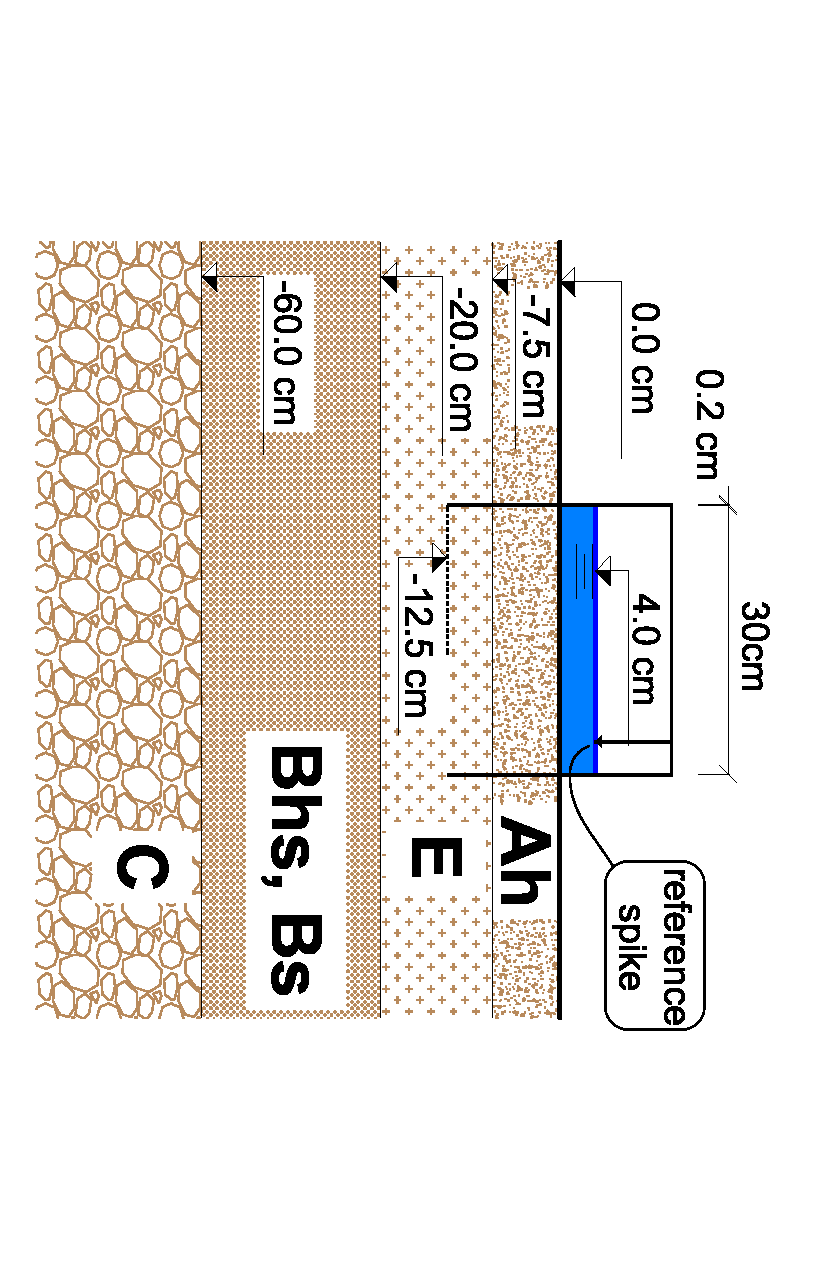
\includegraphics[height=7.5cm]{valec-exp.pdf}}
 \caption{Scheme of the single ring infiltration experiment and the soil layers. }
 \label{experiment}
\end{figure}


For the O+Ah horizon smoothed experimental data from unsteady single ring (SR) infiltration were used as input for inverse modeling of REVG.
The experimental setup was as follows. A steel ring 30~cm in inner diameter, 25~cm in length, and 2~mm in thickness was inserted into the soil to a depth of 12.5~cm, see figure~\ref{experiment}. The depth of ponding was kept approximately at a constant level defined by a reference spike, which was placed 4~cm above the surface of the soil. The average experiment duration was 60~minutes.





A total of 22 SR experiments were conducted on the site. In order to eliminate noise from the experimental values, each SR experiment data set was smoothed with the Swartzendruber analytical model \citep{Swartzendruber}
%add citation to bibtex please: Swartzendruber, D., 1987. A quasi-solution of Richards equation for the downward infiltration of water into soil. Water Resour. Res. 23, 809–817. http://dx.doi.org/10.1029/WR023i005p00809.
of one-dimensional infiltration, which exhibited an excellent fitting quality, with a mean Nash-Sutcliffe model efficiency coefficient  0.9974. The Swartzendruber equation for cumulative infiltration states that
\begin{lineq}
I(t)=\frac{c_0\left(1-\exp\left(-c_1\sqrt{t}\right)\right)}{c_1}+c_2t,
\label{vyhlaz}
\end{lineq}
where $I$ is the cumulative infiltration [$L$], and $c_{0,1,2}$ are parameters. The Swartzendruber model can estimate 1D saturated conductivity and sorptivity of the soil. However, the model does not account for water moving horizontally and therefore overestimates the hydraulic conductivity and gives no information on water retention or unsaturated hydraulic conductivity and is therefore not sufficient. The Swartzendruber model was only considered as an exponential smoothing and interpolating function.


 
A statistical description of the Swartzendruber parameters and their fitting quality is given in~\citep{jacka-site}, see datasets collected on site 3. Representative mean values are as follows: $c_0 =5.130$~cm.hrs$^{-0.5}$, $c_1 = 1.13 \times 10^{-1}$~[-], and $c_2 = 1.858$~cm.hrs$^{-1}$. The parameter set was used to compute the infiltration curve with Eq. \ref{vyhlaz} for the identification of the SHP in the top soil layer.







\subsection{Mathematical model of the field infiltration experiment -- governing equation}%[michal]
\label{goveq}


The field infiltration experiment is characterized by variably saturated conditions. The flux in porous media under variably saturated conditions can be expressed by the Darcy-Buckingham law~\citep{buckingham} \begin{lineq}\label{darcybuck}\vec{q} = -\mathbf{K}(\theta) \nabla H,\end{lineq} where $\vec{q}$ is the volumetric flux [L.T$^{-1}$], $H$ is the total hydraulic head [$L$] defined as $H=h+z$, where $h$ is the pressure head [$L$], $z$ is the potential head [$L$], $\theta$ is the water content [-], and $\mathbf{K}(\theta)$ is the unsaturated hydraulic conductivity  [L.T$^{-1}$]; in general it is a  second order tensor. The relation $\theta(h)$ is referred to as the retention curve~\citep{vangenuchten}.

The geometry of the flow is inherently three-dimensional, but the domain dimension can be reduced by considering the axisymmetric geometry. The law of mass conservation  for incompressible flow in cylindric coordinates is expressed as ~\citep{bear1979}.
\begin{lineq}
\label{conti}
-\frac{\partial V}{\partial t} = \frac{\partial q_r}{\partial r} + \frac{q_r}{r} + \frac{\partial q_{\alpha}}{\partial \alpha} + \frac{\partial q_z}{\partial z} ,
\end{lineq}
where $V$ is the volume function [-],  $r$ is the radial coordinate, $\alpha$ is the angular coordinate,  $z$ is the vertical coordinate, and $q_{r, \alpha, z}$ is the  volume flux [L.T$^{-1}$]. The ring infiltration experiment is characterized by rotational symmetric flow, so the angular derivative vanishes. Then the governing equation for  variably saturated and rotational symmetric flow is obtained by substituting the flux in \eqref{conti} by the Darcy-Buckingham law~\eqref{darcybuck}. Together with the consideration of linear elasticity (expressed by specific storage $S_s$) for a porous medium the variably saturated axisymmetric flow in isotropic media is governed by
\begin{lineq}
\label{richaxi}
\left(\frac{\dd \theta}{\dd h} + S_s\frac{\theta(h)}{\theta_s} \right) \frac{\partial h}{\partial t}  =  \frac{\partial K(h) \frac{\partial H}{\partial z}}{\partial z} + \frac{\partial K(h) \frac{\partial H}{\partial r}}{\partial r} + c(\vec{x})\frac{\partial H}{\partial r},
\end{lineq}
where $S_s$ is the specific storage [L$^{-1}$], $\theta_s$ is the saturated water content [-],  $c(\vec{x})$ is the coefficient of the convection for $r$ coordinate [T$^{-1}$], which is explained below, and the vector $x$ is a vector of the spatial coordinates $\vec{x}=\left( \begin{smallmatrix} r \\ z \end{smallmatrix} \right)$.

 \begin{figure}
\centering
\rotatebox{90}{
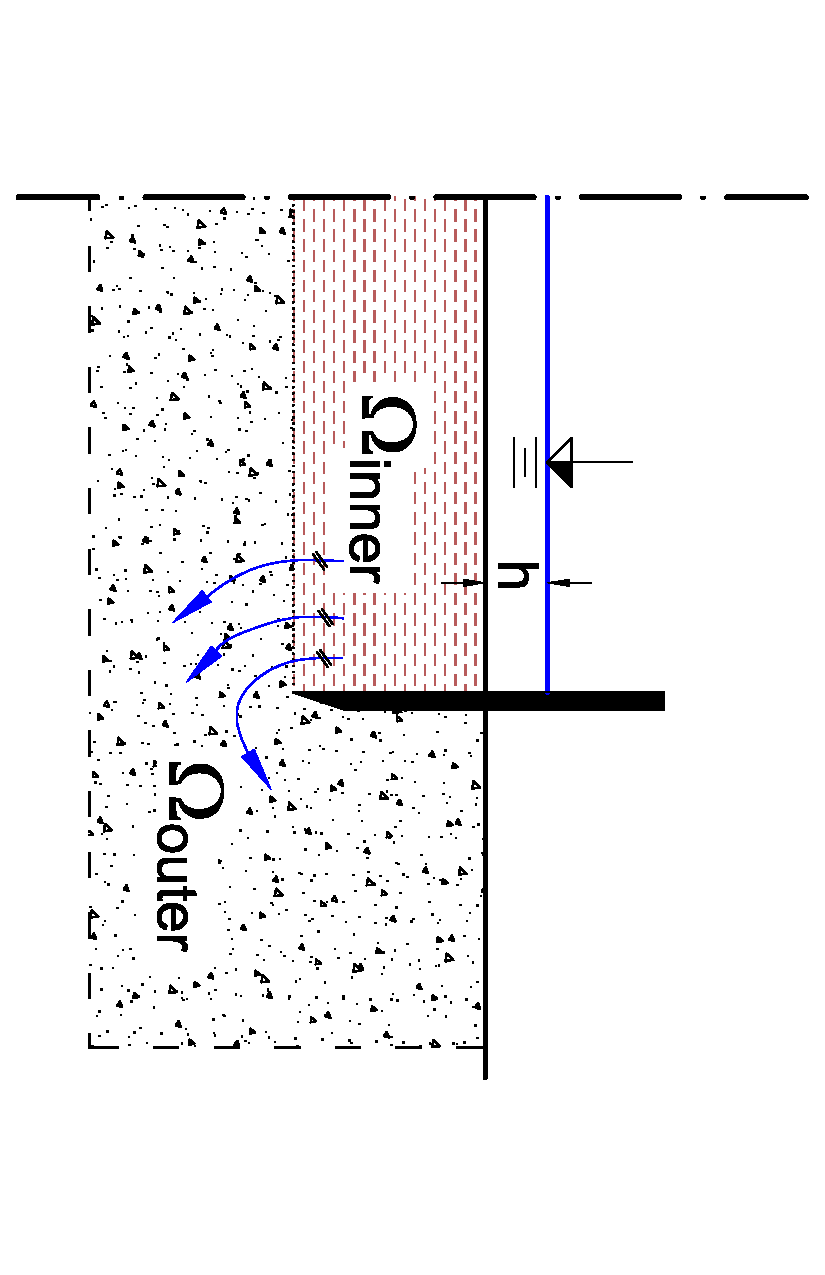
\includegraphics[height=7.5cm]{valcovazk.pdf}}
 \caption{Scheme of the flow domain and the streamlines of infiltration experiment. }
 \label{valecproudy}
\end{figure}

If we consider the model of the infiltration experiment depicted in figure~\ref{valecproudy} with the entire flow domain $\Omega=\Omega_{inner} \cup \Omega_{outer}$, where $\Omega_{outer}$ is the flow domain outside the infiltration ring and $\Omega_{inner}$ is the flow domain within the infiltration ring, exactly as depicted in figure~\ref{valec}. It is then apparent that the streamlines inside subdomain $\Omega_{inner}$ are parallel, but the streamlines outside the infiltration ring (inside $\Omega_{outer}$) are only axisymmetric. The convection coefficient $c(\vec{x})$ is then defined as follows
\begin{lineq}
\label{convect}
c(\vec{x}) = \begin{cases}
	     0 , \quad &\forall \vec{x} \in \Omega_{inner} \\
	     \frac{1}{r}K(h) , \quad &\forall \vec{x} \in \Omega_{outer}.
	    \end{cases}
\end{lineq}
Note that we should avoid using the coordinates, where $r=0$.


\subsection{Domain setup}%[michal]
\label{bccond}
 \begin{figure*}
\centering
\rotatebox{90}{
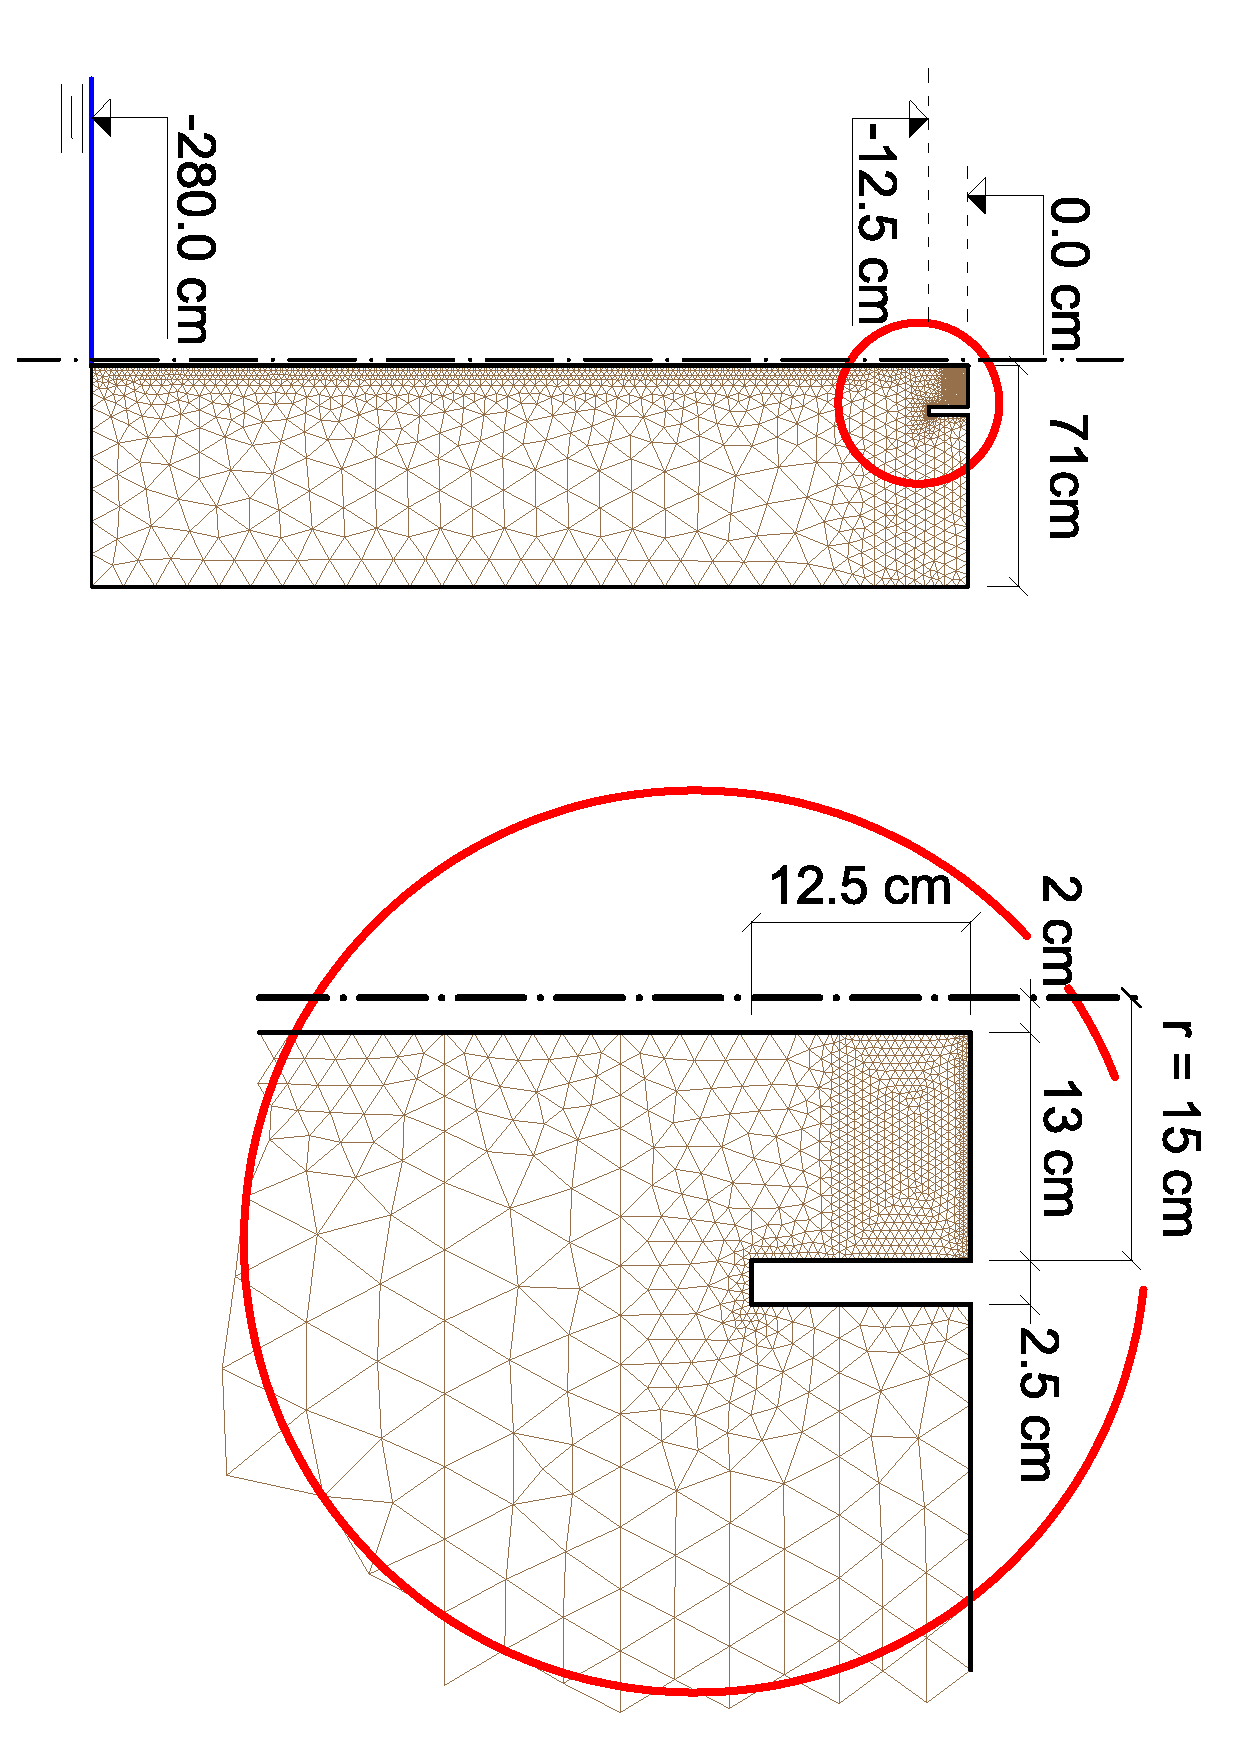
\includegraphics[height=11cm]{infilsit.pdf}}
 \caption{Scheme of the computational domain geometry and domain triangularization.}
 \label{valec}
\end{figure*}


\subsubsection{Domain shape restrictions}

Since \cite{Dusek} mentioned several difficulties with incorrect triangular mesh setup while modeling the SR experiment, we tried to avoid possible numerical issues connected with domains with sharp spikes.

% The governing equation~\eqref{richaxi} will be solved here by linear finite element method, which is a subset of variational methods. Using standard setup the solution $H$ of~\eqref{richaxi} will be taken from Sobolev functional space defined for functions on Lipschitz bounded domains~\citep{braess, pum}.

%reseni rovnice bylo ve std pojeti, reseni ze sobolevova prostoru funkci definovanych na oblasti z lips hranici
Sudden changes in domain shapes, spikes and discontinuities yield numerical difficulties (e.g. the Lipschitz boundary restrictions~\citep{braess}).
In order to avoid computational difficulties during the automatic calibration procedure the infiltration ring thickness was oversized  to 2.5~cm. It is obvious that the real ring thickness is much smaller (in our case 2~mm), but using the real ring thickness yields possible numerical issues.  It is expected, that oversizing the ring thickness does not significantly affect the fluxes through the top Dirichlet boundary, which is the only important part of the solution of~\eqref{richaxi} for our calibration process.


\subsubsection{Stability restrictions of convection dominant problems}
\label{restrconvect}

The equation \eqref{convect} refers to coefficient  of the first order derivative term in~\eqref{richaxi}, and so the well known stability restrictions for the numerical solutions of the convection-diffusion problems appear here~\cite{zienkiewicz1976}.
The Peclet number representing the numerical stability of convection-diffusion problems is defined as~\citep{knobloch2008} 
\begin{lineq}
\label{peclet-std}
Pe = \frac{c \Delta x}{2 D},
\end{lineq}
where $c$ is the convection coefficient defined in~\eqref{convect}, $\Delta x$ is the discretization step, and $D$ is the diffusion (for isotropic setup). Based on the definitions given above, equation~\eqref{peclet-std} can be formulated as
\begin{lineq}
Pe =  \frac{\frac{1}{r}K(h) \Delta x}{2K(h)} = \frac{\Delta x}{2r}.
\end{lineq}
Since our mesh is triangular, $\Delta x$ can be roughly assumed to be the greatest triangle altitude (since we assume some mesh quality properties). Then a sufficient distance from the axis of anisotropy is such that the Peclet number is sufficiently low. If we want to make our computation free of the well known spurious oscillations~\cite{zienkiewicz1976, roos-layers}, a sufficiently low Peclet number $Pe\le 1$ is required. Therefore, the distance from the axis of anisotropy is given by the domain discretization step at the left hand side boundary. The selected discretization step at the left hand side boundary was assumed as $\Delta x=2$~cm. The domain was therefore detached by 2~cm from the axis of anisotropy, and thus the Peclet number was 0.5 only.












\subsubsection{Initial and boundary condition setup}


The goal of the model was to achieve cumulative infiltration -- the cumulative flux over the top Dirichlet boundary.
The computational domain is depicted in figure~\ref{valec} together with the discretization mesh. The location of the top boundary was natural -- the soil surface. Inside the ring, a Dirichlet condition defines the ponding depth; outside the infiltration ring a Neumann condition defines the no-flow boundary. Locating the bottom boundary was more problematic. We consider following commonly used options:
\begin{itemize}
\item the no-flow boundary (Neumann)
\item the free drainage boundary (Neumann)
\item the groundwater level - zero pressure head (Dirichlet)
\end{itemize}
It is apparent that the wetting front originating from our infiltration experiment affects the soil column only to a certain depth. Defining the Neumann no-flow boundary at a sufficient depth would therefore probably not have a significant effect on the derivative of the solution of \eqref{richaxi} at the top boundary. At the same time, the only physically acceptable location of the no-flow boundary is the groundwater table. The second option -- the free drainage boundary -- would be completely incorrect for any depth. The free drainage boundary defines fluxes that probably do not appear in our system at all.  If we consider the initial condition to represent a hydrostatic state, and so \begin{lineq} \frac{\partial h}{\partial z}(x) = -1, \quad \forall x \in \Omega .\end{lineq} The free drainage boundary condition, which is defined as
\begin{lineq}
\frac{\partial h}{\partial \vec{n}}(x) = 0, \quad \forall (x,t) \in \Gamma_{\mbox{\footnotesize free drainage}} \times [0,T).
\end{lineq}
is in a conflict with the initial condition (since the outer normal vector $\vec{n} = \left(\begin{smallmatrix} &0 \\ -&1 \end{smallmatrix} \right)$), which is again physically incorrect, and produces extra computational costs. The computational process, that is produced at the bottom boundary in the beginning of the simulation with such a boundary setup, originates from the initial and boundary condition mismatch, and has no physical meaning.

It turns out that the only physically correct boundary condition for the bottom boundary is either the Neumann no-flow boundary or Dirichlet boundary both at the groundwater table. The average depth of the groundwater table is approximately -280~cm below the surface. With this particular setup the domain became extremely narrow and deep, see figure~\ref{valecbc}.


As discussed in \ref{restrconvect} the left hand side boundary was located at $r=2$~cm. The right hand side boundary was located at a distance $r=73$~cm and 60~cm from the infiltration ring. 

 \begin{figure}
\centering
\rotatebox{90}{
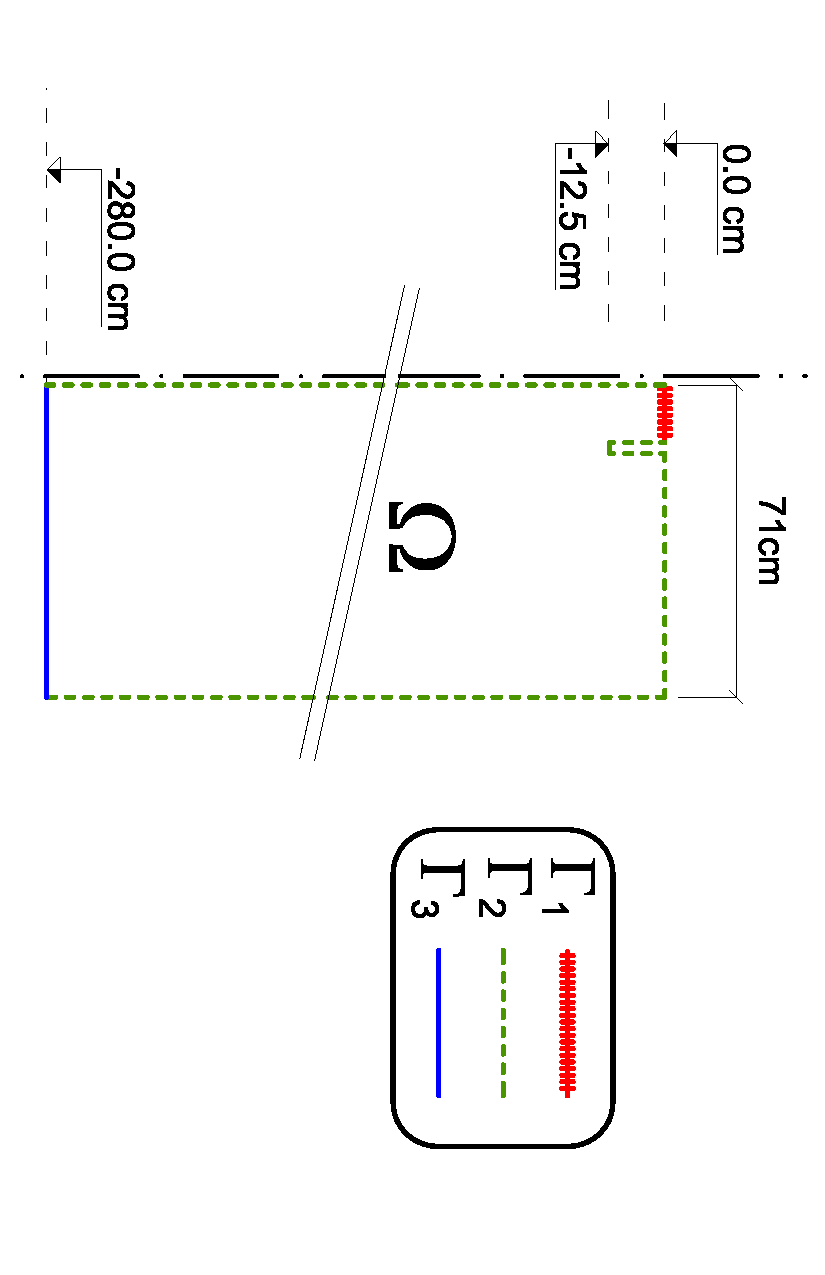
\includegraphics[height=8cm]{schemabc.pdf}}
 \caption{Scheme of the computational domain geometry and the domain boundaries.}
 \label{valecbc}
\end{figure}


The locations of the domain boundaries are depicted in figure~\ref{valecbc}. The boundary conditions are specified as follows (with the reference level $z=0$ located at the top boundary)
\begin{lineq} 
\begin{split}
h(x,t) &= 4 \; \mbox{cm} \Rightarrow H(x,t) = 4 \; \mbox{cm}; \quad \forall (x,t) \in \Gamma_1 \times [0,T), \\
\frac{\partial H}{\partial \vec{n}} &= 0; \quad \forall (x,t) \in \Gamma_2 \times [0,T), \\
h(x,t) &= 0  \; \mbox{cm}  \; \Rightarrow \; H(x,t) = -280.0  \; \mbox{cm}; \quad \forall (x,t) \in \Gamma_3 \times [0,T).
\end{split}
\end{lineq}
where $T$ is the simulation end time [T], and $\vec{n}$ is the boundary normal vector.

The initial condition was assumed as a steady state  solution  of \eqref{richaxi} with the boundary $\Gamma_1 \cup \Gamma_2$ assumed as a no-flow boundary -- thus the entire domain $\Omega$ was considered to be in hydrostatic state. The initial condition states that 
\begin{lineq}
H(x) = -280.0 \; \mbox{cm}; \quad \forall x \in \Omega,
\end{lineq}
and thus $\frac{\partial h}{\partial z} = -1$.




\subsection{Optimization}

\subsubsection{Objective function} %[michal]
\label{objdef}

The soil hydraulic parameters (SHP) of the top soil that will be identified were specified in section~\ref{shp}.
Since the parameters will be identified using a stochastic method, we have to introduce a physically reasonable range for each parameter. The ranges for the SHP are specified in table~\ref{rozsahy}.

\begin{table*}[ht]
\begin{center}
\caption{Ranges of SHP ($\vec{p}_{max}$ and $\vec{p}_{min}$) for identifying the SHP in the top-soil layer for {\it refinement level} $r_f=0$. Note that the initial ranges are extremely broad especially for the saturated water content $\theta_s$. This broad range was selected in order to explore the uniqnuess
of the REVG inverse model of SR experiment
 even beyond the physically acceptable solutions. }
\fs
\begin{tabular}{c | c| c| c| c}
\toprule
% Ranges of depths, horizon(s)&\multicolumn{4}{c}{Input values for inverse modelling}\\ \cline{2-5}
$\theta_s$ [-]&$\alpha$ [cm$^{-1}$]&n [-]& $K_s$ [m.s$^{-1}$] & $S_s$ [m$^{-1}$] \\ \hline
\toprule
0.25 -- 0.90 & \num{0.01e-2} -- \num{5.0e-2} & 1.05 -- 4.5 & 0.300 -- 300.0 & 0.0 -- 0.1 \\
\toprule
\end{tabular}
\label{rozsahy}
\end{center}
\end{table*}

The objective function is defined in the following paragraph.


Let $\bar{I}(\vec{p},t)$ be the cumulative infiltration obtained from solving the mathematical model~\eqref{richaxi} bounded by the initial and boundary conditions  defined in section~\ref{bccond} for a certain vector of SHP parameters $\vec{p}$ considered as
\begin{lineq}\bar{I}(\vec{p},t) = \frac{\int\limits_0^t \int\limits_{\Gamma_1}-K \frac{\partial H}{\partial \vec{n}}(t)  \dd \Gamma_1 \dd t}{\int\limits_{\Gamma_1} \dd \Gamma_1}.\end{lineq}
Let $I(t)$ be the cumulative infiltration defined by \eqref{vyhlaz} with parameters given in section~\ref{krivka}. 
Then the objective function was defined for three different criteria in order to avoid ill-posed objective function definition.

The objective functions were defined as follows:
\begin{enumerate}[label={\bf \Roman*}.]
\item First criterion $\Psi_1$ was defined as $L_2$ norm of the difference between the  experimental and model data and thus
\begin{lineq}
\label{objektiva1}
\Psi_1 (\vec{p}) = \sqrt{\int\limits_0^{T_{end}} \left( \bar{I}(\vec{p},t) - I(t) \right)^2 \dd t},
\end{lineq}
where $T_{end}$ is the final simulation time [$T$], which is indeed the root mean square error (RMSE) for continuous functions. 
\item Second criterion was the $L_{\infty}$ norm of the difference between the experimental and model data and thus
\begin{lineq}
\label{objektiva2}
\Psi_2 (\vec{p}) = \mathrm{sup} \left( \sqrt{\left( \bar{I}(\vec{p},t) - I(t) \right)^2} \right), \quad  t \in (0, T_{end}).
\end{lineq}
\item Third criterion was considered as the difference between the infiltration rates (final derivatives) between the model data and the experimental data
\begin{lineq}
\label{objektiva3}
\Psi_3 (\vec{p}) =  \sqrt{\left( \frac{\dd \bar{I}(\vec{p},T_{end})}{\dd t} - \frac{\dd I(T_{end})}{\dd t} \right)^2}.
\end{lineq}


\end{enumerate}

We conducted multi-objective optimization. However, it is apparent that minimizing the objective function~\eqref{objektiva1} also minimizes the objective functions~\eqref{objektiva2} and \eqref{objektiva3}. The aim of this multi-objective definition was to improve the conditioning of this inverse problem. If we only considered the objective function~\eqref{objektiva1}, then we were probably able to obtain the same solution as with this multi-objective definition with slower convergence of optimization procedure only (the selection of the optimization algorithm will be explained in the following section~\ref{optima}). This multi-objective function definition is based on our experience from previous attempts of inverse analysis of this infiltration problem.



\subsubsection{Optimization algorithm}%[matej]
\label{optima}

In this contribution we used the modified genetic algorithm GRADE \citep{grade,Kucerova:2007:PHD} supported by niching method CERAF \citep{Hrstka} enhancing the algorithm with
memory and restarts. GRADE is a real-coded genetic algorithm combining the ideas of genetic operators: cross-over, mutation and selection taken from the standard genetic algorithm and differential operators taken from differential evolution. When GRADE converges, the current position of the optimization algorithm is marked as a local extreme and a forbidden area is built around it in order to forbid the optimization algorithm to fall into the same local extreme again. The main setting of the optimization procedure was as follows: the population of the genetic algorithm contains 30 independent solutions, the whole identification stops after 20.000 objective function evaluations and a local extreme was marked after 600 evaluations without any improvement.


% \subsubsection{Multi-objective Optimization}
% !!!!!!add connections
 In this contribution Average Ranking (AR) \citep{Leps:2007} was used to deal with multi-objective definition. It sums ranks of the objective functions instead of the objective functions' values. Therefore, no weights are needed, however, the Pareto-dominance is not preserved as described in \cite{vitingerova:2010}. An application of the AR algorithm to parameters identification can be found in \cite{Kuraz:2010:JCAM}. 


\subsection{Numerical solution and computational issues}
\label{trapoty}

Equation~\eqref{richaxi} was implemented into the DRUtES library~\citep{drutes}. It is an object-oriented library written in Fortran 2003/2008 standard for solving nonlinear coupled convection-diffusion-reaction type problems. The problem was approximated by the linear finite element method for spatial derivatives and Rothe's method for temporal derivatives. The nonlinear operator was treated with the Schwarz-Picard method -- an adaptive domain decomposition  ($dd$-adaptivity) -- with the ability to activate and deactivate subregions of the computational domain sequentially ~\citep{mojecomp, mojejcam2, mojeamc2}.



 The domain was non-uniformly discretized by a triangular mesh. The smallest spatial step was considered for the top layers inside the infiltration ring, close to the Dirichlet boundary. The mesh is depicted on figure~\ref{valec}. The minimum spatial length was 0.5~cm, and the maximum spatial length was 20~cm. The domain was discretized with 2097 nodes and 3861 elements. The coarse mesh for the $dd$-adaptivity method was a uniform quadrilateral mesh with elements 17.75$\times$28.0~cm, i.e. a total of 40 coarse elements and 55 nodes. The purpose of the coarse mesh is to organize the elements of the domain triangularization into so-called clusters, which form a basic unit for the adaptive domain decomposition used here for solving the nonlinear problem, details can be found in~\citep{mojeamc2}.

 
 The spatial and temporal discretization of \eqref{richaxi} leads to sequential solutions of systems of non-linear equations, see e.g.~\citep{mojecomp}. The system was linearized as discussed in~\citet{mojeacta, mojeamc}, and so the numerical solution requires an iterative solution of 
\begin{lineq}
\label{matice}
\mathbf{A}(\vec{x}_l^k) \vec{x}_l^{k+1} = \vec{b}(\vec{x}_l^k),
\end{lineq}
where $k$ denotes the iteration level, and $l$ denotes the time level, until \begin{lineq} \label{picard} ||\vec{x}_l^{k+1} - \vec{x}_l^k||_2 < \varepsilon , \end{lineq} where $\varepsilon$ is the desired iteration criterion.  It is apparent that the number of required  iterations depends on the $\varepsilon$ criterion. 


The method~\eqref{matice} degenerates into a kind of semiexplicit approximation if the error criterion $\varepsilon$ was "infinitely huge" -- it means taken from the extended real numbers, $\varepsilon \in {\overline {\mathbb {R} }}$, and assigned as $\varepsilon = + \infty$. This semiexplicit approximation is denoted as
\begin{lineq}
\label{matice2}
\mathbf{A}(\vec{x}_{l-1}) \vec{x}_l = \vec{b}(\vec{x}_{l-1}).
\end{lineq}
 This semiexplicit method always requires just a single outer iteration. With a short time step the method converges to the exact solution. For inappropriate time steps, the method diverges from the exact solution faster than the method~\eqref{matice}. Nonetheless, the method~\eqref{matice2} is free of possible issues related to the convergence of the nonlinear operator.



\section{Automatic calibration methodology}%[michal]




The infiltration flux is obtained from the numerical derivative of the solution of \eqref{richaxi},  and  it is known that inaccurate approximation of the capacity term (time derivative term) yields inaccurate mass properties~\citep{celia}. We are aware of the possible impact of spatial and temporal discretization on the identified SHP values. We are also aware of possible difficulties with convergence of the linearized discrete system~\eqref{matice} for certain combinations of SHP parameters during the automatic calibration, as discussed by~\cite{beven2003-uncertain}.

Following the concerns about  effects of numerical treatment for the identified values of SHP parameters a specific  automatic calibration methodology was proposed. The technique is explained in brief in figure~\ref{flowchart}, and  details are given in the following paragraph.

Before we start with automatic calibration description, the following nomenclature will  be defined % I really wanted to say here Let us define :)
\begin{description}
\item[$\vec{p}$] -- vector of SHP parameters, vector contains the values of $\alpha$, $n$, $\theta_s$, $K_s$, $S_s$,
\item[$r_f$] -- "refinement level", the problem is treated with different spatial and temporal discretization setups, each setup is denoted by value of $r_f$ index,
\item[$\vec{p}_{max,min}^{r_f}$] -- maximal, resp. minimal values of SHP parameters,
\item[$i_e$] -- local extreme index,
\item[$\Delta(\vec{x})$] -- spatial discretization (mesh density, mesh is non-uniform).
\end{description}

 


\begin{figure*}
\centering
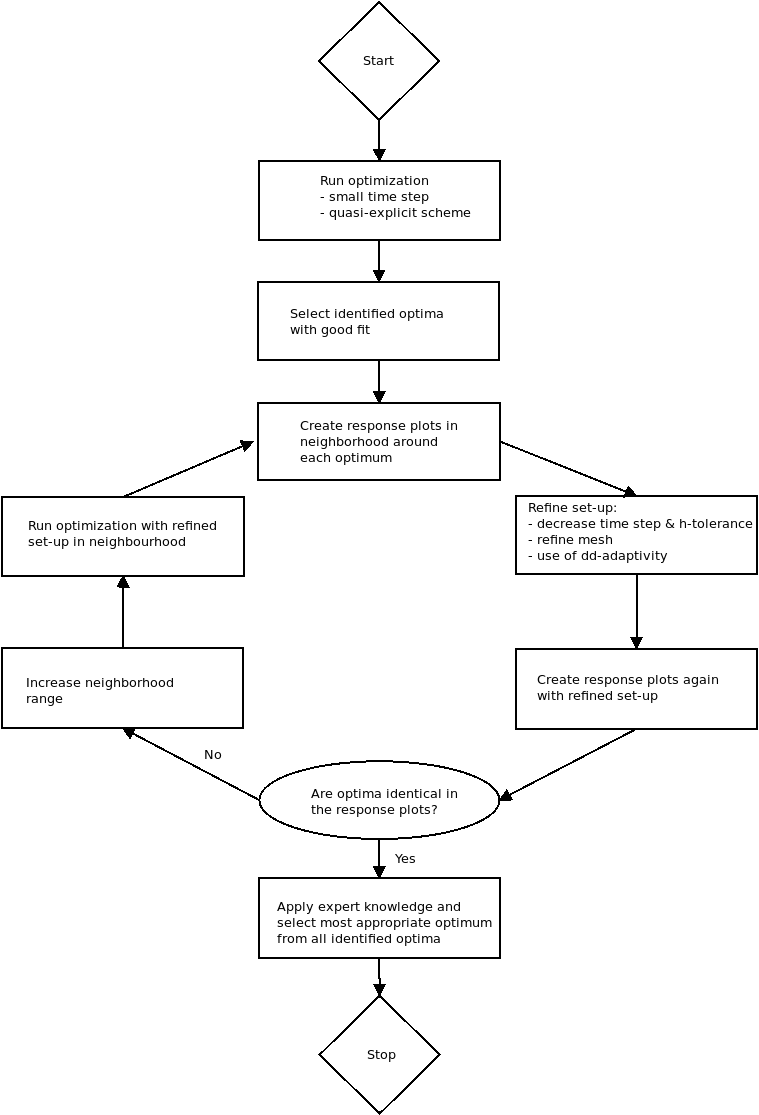
\includegraphics[width=12cm]{flowchart/Flow_chart_cb_new.png}
\caption{The proposed methodology for the automatic calibration avoiding effects of numerical treatment for the identified SHP values.}
\label{flowchart}
\end{figure*}

The calibration algorithm is described as follows:

 \begin{enumerate}[label=({\bf \roman*})]
\item {\bf Do} initial calibration with semiexplicit treatment of~\eqref{matice} ($\varepsilon \leadsto +\infty$), $r_f$=0,  vectors $\vec{p}_{max,min}^{r_f}$ are taken from table~\ref{rozsahy}. 
\item {\bf If} the problem is multimodal\begin{itemize} \item {\bf Then} sequence of vectors $\vec{p}^{i_e}_{r_f}$ is generated. \end{itemize} 
\item {\bf Do} validation: \begin{itemize} \item select local extremes with good fitting qualities, \item increase $r_f=r_f+1$ as follows 
                  \begin{lineq}
                  \label{coeffs}
                  \begin{split}
                  \Delta(\vec{x})^{r_f}  &= \frac{\Delta(\vec{x})^{r_f-1}}{2}, \\
                  \varepsilon^{r_f} &= 10^{-3} \; \mbox{cm} \quad  \mbox{if} \; r_f = 1, \; \; \mbox{else} \quad \varepsilon^{r_f} = \frac{\varepsilon^{r_f-1}}{10}, \\
                  t_{init}^{r_f} &=  \frac{t_{init}^{r_f-1}}{10} \; \mbox{hrs} .
                  \end{split}
                  \end{lineq}
\item create a response plot of the objective function~\eqref{objektiva1} for current $r_f$ and $r_f-1$ in the neighborhood defined as 
\begin{lineq}
\begin{split}
\vec{p}^{i_e, r_f}_{max} &= 1.20\vec{p}^{i_e}, \\
\vec{p}^{i_e,r_f}_{min} &= 0.70\vec{p}^{i_e}. 
\end{split}
\end{lineq}
\end{itemize}

\begin{enumerate}
\item {\bf Validation methodology:}

  \begin{enumerate}
    \item \label{val} Compare the response 
   plots for the selected local extreme $i_e$ created with discretization $r_f$ and $r_f-1$.
    \item \label{cond} {\bf If} the response plots differ significantly.
   \begin{itemize}%[label=(\subscript{b}{\arabic*})]
    \item {\bf Then} do the calibration at parameter range: \begin{lineq} \begin{split} \vec{p}_{max} &= 1.2\vec{p}^{i_e,r_f-1}, \\   \vec{p}_{min} &= 0.8\vec{p}^{i_e,r_f-1 }. \end{split}\end{lineq} New sets of vectors  $\vec{p}_{r_f}^{i_e}$ will be generated.
    \item \label{ll2} Increase the discretization level $r_f$ as $r_f=r_f+1$, perform the update~\eqref{coeffs}, return to~\ref{val}, and check the condition~\ref{cond}.
    \end{itemize}
    \item {\bf else}
    \begin{itemize}%[label=(\subscript{c}{\arabic*})]
    \item Exit the calibration process.
    \end{itemize}
  \end{enumerate}
\end{enumerate}
\end{enumerate}
% In the second stage the unknown SHP parameters will be reduced and the automatic calibration using the initial mesh together with the simple quasi-explicit approximation~\eqref{matice2} will proceed.
% The unknown SHP parameters will be sequentially reduced in the following order until just a single extreme will be identified.
% \begin{enumerate}[label=({\bf \Roman*})]
% \item $S_s$ -- specific storage is often neglected for the unsaturated zone, and thus for the first unknown parameter reduction will be assigned $S_s=0\;\mbox{m}^{-1}$
% \item $\theta_s$ -- water content is often easy to measure directly, despite there are no available data for top soil layer, let's presume $\theta_s = 0.6.$
% \item $K_s$ -- if the identifiability of the inverse model will require also reduction of $K_s$, then this inverse task became inappropriate for any further analyses, and the conducted SR measurements will be declared as non-identifiable setup for SHP parameters.
% \end{enumerate}


The following sections will further explain the definition of the objective function and the parameter identification algorithm.




 
 

 



\section{Results and discussion} 




\subsection{Benchmark evaluations}
 \label{benchmarks}
 
The purpose of this benchmark example was to demonstrate, whether this class of problem -- identification of SHP parameters from cumulative flux measured at Dirichlet boundary -- can be affected by multimodality.


 For simplicity only a one-dimensional Richards equation problem was considered here.  Dirichlet boundary conditions were presumed for both boundaries. The model setup state as follows. Computational domain was $\Omega=(0,100\,\mathrm{cm})$, and the boundary and initial conditions stated as follows
 \begin{lineq}
 \begin{split}
 h(x,t) &= 0\, cm, \quad \forall (x,t) \in \Gamma_{bot} \times  t \in [0, T_{end}) \\ 
  h(x,t) &= 0\, cm, \quad \forall (x,t) \in \Gamma_{top} \times  t \in [0, T_{end}) \\ 
  H(x,t_0) &= 0\, cm , \quad \forall x \in \Omega,
  \end{split}
\end{lineq}
 where $\Gamma_{bot}=0.0$ cm, $\Gamma_{top}=100.0$ cm, and $T_{end}=$\num{e-1}~hrs. Two distinguished soil types were considered here -- clay loam and sand, the parameters were obtained from~\citep{retc}, and are given in table~\ref{tab:bench}
 

 
  The computational domain $\Omega$ was uniformly discretized with $\Delta x$=0.5~cm, the initial time step was $\Delta t$=\num{e-7}~hrs, and the error criterion from~\eqref{picard} for solving the nonlinear system~\eqref{matice} was   $\varepsilon$=\num{e-3}~cm.
 
 The reference solutions both for sand and gravel media were obtained from  cumulative flux over the top Dirichlet boundary $\Gamma_{top}$.
 
For the given reference solutions the inverse modeling algorithm described in section~\ref{optima} was employed for searching the original SHP parameters in broad ranges given in table~\ref{rozsahy}. 
In order to avoid effects of numerical treatment of the Richards equation, the numerical solver had exactly the same configuration as the one used for the reference solution. 
 




\begin{table*}[]
\centering
\caption{Results of the benchmark problem. The grey highlighted rows refer to the physically acceptable solution of this benchmark inverse problem, and the red highlighted rows contain the exact solution of this inverse problem.}
\label{tab-benchres}
\footnotesize
\begin{tabular}{|c|c|c|c|c|c|c|c|}
\hline
\multicolumn{3}{|c|}{\cellcolor[HTML]{34CDF9}}                                                                                                                        & \multicolumn{4}{c|}{parameters}                                                                                                                                                                                                                            &                                             \\ \cline{4-7}
\multicolumn{3}{|c|}{\multirow{-2}{*}{\cellcolor[HTML]{34CDF9}}}                                                                                                      & $\alpha$ [cm$^{-1}$]                                          & $n$ [-]                                                      & $\theta_s$ [-]                                               & $K_s$ [cm.hrs$^{-1}$]                                        & \multirow{-2}{*}{RMSE error}                \\ \hline
                                     & \multicolumn{2}{c|}{\cellcolor[HTML]{CB0000}{\color[HTML]{FFFFFF} \textbf{exact solution}}}                                    & \cellcolor[HTML]{CB0000}{\color[HTML]{FFFFFF} \textbf{0.019}} & \cellcolor[HTML]{CB0000}{\color[HTML]{FFFFFF} \textbf{1.31}} & \cellcolor[HTML]{CB0000}{\color[HTML]{FFFFFF} \textbf{0.41}} & \cellcolor[HTML]{CB0000}{\color[HTML]{FFFFFF} \textbf{6.24}} & \cellcolor[HTML]{34CDF9}                    \\ \cline{2-8} 
                                     &                                                                                           & \cellcolor[HTML]{C0C0C0}\textbf{1} & \cellcolor[HTML]{C0C0C0}0.020                                 & \cellcolor[HTML]{C0C0C0}1.321                                & \cellcolor[HTML]{C0C0C0}0.395                                & \cellcolor[HTML]{C0C0C0}6.226                                & \cellcolor[HTML]{C0C0C0}\num{0.04787}       \\ \cline{3-8} 
                                     &                                                                                           & \textbf{2}                         & 0.012                                                         & 1.050                                                        & 0.250                                                        & 7.011                                                        & \num{0.2830367232}                          \\ \cline{3-8} 
\multirow{-4}{*}{\textbf{clay loam}} & \multirow{-3}{*}{\textbf{\begin{tabular}[c]{@{}c@{}}identified\\ solutions\end{tabular}}} & \textbf{3}                         & \num{0.00012796}                                              & 1.146                                                        & 0.900                                                        & 94.904                                                       & \num{0.3724314113}                          \\ \hline
\multicolumn{8}{|l|}{\cellcolor[HTML]{656565}}                                                                                                                                                                                                                                                                                                                                                                                                                                   \\ \hline
                                     & \multicolumn{2}{c|}{\cellcolor[HTML]{CB0000}{\color[HTML]{FFFFFF} \textbf{exact solution}}}                                    & \cellcolor[HTML]{CB0000}{\color[HTML]{FFFFFF} \textbf{0.145}} & \cellcolor[HTML]{CB0000}{\color[HTML]{FFFFFF} \textbf{2.68}} & \cellcolor[HTML]{CB0000}{\color[HTML]{FFFFFF} \textbf{0.43}} & \cellcolor[HTML]{CB0000}{\color[HTML]{FFFFFF} \textbf{29.7}} & \cellcolor[HTML]{34CDF9}                    \\ \cline{2-8} 
                                     &                                                                                           & \textbf{1}                         & 0.039                                                         & 1.050                                                        & 0.250                                                        & 35.563                                                       & \num{0.02977800386}                         \\ \cline{3-8} 
                                     &                                                                                           & \textbf{2}                         & 0.026                                                         & 1.087                                                        & 0.587                                                        & 37.877                                                       & \num{0.02405719725}                         \\ \cline{3-8} 
\multirow{-4}{*}{\textbf{sand}}      & \multirow{-3}{*}{\textbf{\begin{tabular}[c]{@{}c@{}}identified\\ solutions\end{tabular}}} & \cellcolor[HTML]{C0C0C0}\textbf{3} & \cellcolor[HTML]{C0C0C0}0.154                                 & \cellcolor[HTML]{C0C0C0}2.654                                & \cellcolor[HTML]{C0C0C0}0.460                                & \cellcolor[HTML]{C0C0C0}30.145                               & \cellcolor[HTML]{C0C0C0}\num{0.02198515637} \\ \hline
\end{tabular}
\end{table*}

Results of the benchmark problem are given in table~\ref{tab-benchres}. For these two different soil types involved  the inverse modeling algorithm has found several local optima, and the low value of an objective function doesn't necessarily  point to the correct solution. Thus the problem is multi-modal. Several distinct SHP parameter sets can lead to acceptable solutions. However, the most distinct SHP parameter is the saturated water content $\theta_s$. It turns out that an expert knowledge is required here, to select an acceptable solution of this inverse problem.  




% clay with original settings
%  0.020367, 1.3219, 0.39551, 6.2261  0.04787
% 0.011519, 1.05, 0.2502, 7.0108 0.2830367232
%  0.00012796, 1.1462, 0.9, 94.904 0.3724314113
 
%  clay with semi-explicit
% 0.019941, 1.3504, 0.46568, 7.005 0.560637688
%  0.094183, 3.7989, 0.25003, 3.8626 1.290496494
% 0.019983, 1.35, 0.26555, 6.9927 0.6542315846

% sand with original settings
% 0.039412, 1.0502, 0.25018, 35.563 0.02977800386
% 0.026293, 1.0872, 0.58662, 37.877 0.02405719725
% 0.154 & 2.6543 &  0.46 & 30.145 0.02198515637 

%sand with semiexplicit
%  0.042468, 1.1269, 0.25569, 69.785 0.0157830282
% 0.12224    2.45494       0.35    32.6334 0.0139951908



 The local extremes for the refinement level $r_f=0$ are given in table~\ref{shp-vysledky}, where the gray lines refer to local extremes with bad fitting properties (extremes 1-5), the local extremes 6-8 refer to inverse model solutions with good fitting properties. The results were visually inspected. An example of bad fitting dataset is depicted on figure~\ref{rf0samples} - left, and the example of the good fitting dataset is depicted on figure~\ref{rf0samples} - right. Solution for each dataset is  given in Appendix. Complete settings specifications for each $r_f$ level involved here are given in table~\ref{tab:rfset}.




\begin{table*}[]
\centering
\fs
\caption{Settings for different $r_f$ levels. Computer architecture  32-core Intel(R) Xeon(R) CPU E5-2630, bogomips 4801.67, objective functions were evaluated in parallel.}
\label{tab:rfset}
\begin{tabular}{|c||c|c|c|c|c|c|}
\hline
\begin{tabular}[c]{@{}c@{}}$r_f$ \\ level\end{tabular} & \begin{tabular}[c]{@{}c@{}}Picard criterion\\ $\varepsilon$ [cm] \end{tabular} & \begin{tabular}[c]{@{}c@{}}number of \\ nodes\end{tabular} & \begin{tabular}[c]{@{}c@{}}number of\\ elements\end{tabular} & \begin{tabular}[c]{@{}c@{}}initial\\ $\Delta t$ [hrs] \end{tabular} & \begin{tabular}[c]{@{}c@{}}number of \\ objective function\\ evaluations\end{tabular} & \begin{tabular}[c]{@{}c@{}}CPU time  for \\  objective function\\ computation [min]   \end{tabular} \\ \hline  \hline
0                                                      & $\leadsto +\infty$                                                       & 2097                                                       & 3861                                                         & \num{e-6}                                                    & 40 000                                                                                & 3                                                                                                \\ \hline
1                                                      & \num{e-3}                                                                & 4503                                                       & 8488                                                         & \num{e-7}                                                    & 1 000                                                                                 & 20                                                                                               \\ \hline
2                                                      & \num{e-4}                                                                & 9637                                                       & 18588                                                        & \num{e-8}                                                    & 1 000                                                                                 & 60                                                                                               \\ \hline
\end{tabular}
\end{table*}



\begin{table*}
\begin{center}
\caption{Identified local extremes of Pareto front during the first run of parameter search procedure.}
\fs
\begin{tabular}{l || c c c c c  }
\toprule
no. & $\alpha$ [cm$^{-1}$] & $n$ [-] & $\theta_s$ [-] & $K_s$ [cm.hrs$^{-1}$] & $S_s$  [cm$^{-1}$] \\ \hline \hline
\rowcolor{gray}{\bf 1} & \num{2.447e-4} &  2.45 & 0.25 & \num{0.025} & \num{0.419e-2}   \\ 
\rowcolor{gray}{\bf 2} & \num{0.101e-2} & 0.6517 &  0.271 & \num{1.092} &  \num{2.879e-2}  \\ 
\rowcolor{gray}{\bf 3} & \num{1.840e-2} & 2.098 & 0.353 & \num{1.092} & \num{1.845e-4} \\
\rowcolor{gray}{\bf 4} & \num{0.157e-2} & 1.968 & 0.720 & \num{2.07} & \num{1.053e-5}  \\ 
\rowcolor{gray}{\bf 5} & \num{0.150e-2} & 1.586 & 0.720 &  \num{1.093} &  \num{7.641e-3}  \\ \hline \hline
\rowcolor{white}{\bf 6} & \num{0.258e-2} & 2.152  & 0.401 &  \num{1.095} & 0  \\ 
\rowcolor{white}{\bf 7} & \num{0.3802e-2} & 1.279 & 0.594 &  \num{1.165} & 0  \\ 
\rowcolor{white} {\bf 8} & \num{0.255e-2} & 1.384 & 0.254 &  \num{1.119} &  \num{1.922e-4}  \\ \hline
\toprule
\end{tabular}
 \label{shp-vysledky}
\end{center}
\end{table*}


\begin{figure}
\rotatebox{-90}{
{\includegraphics[height=7cm]{images/badfit/2.eps}}}
\rotatebox{-90}{
{\includegraphics[height=7cm]{images/hezky/1.eps}}}
\caption{Left: Local extreme 2 -- bad fitting properties, Right: Local extreme 5 -- good fitting properties.}
\label{rf0samples}
\end{figure}

In the next step the refinement level was increased, new mesh was generated.

For the local extreme 6, the refined numerical treatment $r_f=1$ has not affected the objective function, the figure~\ref{objfnc6} depicts two examples of the scatter plots -- for the parameter $\alpha$ and $n$. The scatter plots of all parameters are given in Appendix. The response for the $\alpha$ parameter (figure \ref{objfnc6} - left) seems adequate, which was not the case of $n$ parameter  (figure \ref{objfnc6} - right). It turns out that for this parameter set the objective function exhibits poor local sensitivity. However, this was not the case of the other local extremes, see figure~\ref{objfnc6.2} - left. 

The local extreme 8 is characterized by nonzero specific storage $S_s$. However, if we look closer to the scatter plot~\ref{objfnc6.2} - right, it becomes apparent, that the specific storage should vanish even for this parametric set. Both local extremes 7 and 8 exhibit similar local sensitivity and similar response for changing the $r_f$ level, as the one depicted in figure~\ref{objfnc6.2} - right.




\begin{figure}
\rotatebox{-90}{
{\includegraphics[height=7cm]{data/objvals/alpha-4.eps}}}
\rotatebox{-90}{
{\includegraphics[height=7cm]{data/objvals/n-4.eps}}}
\caption{Scatter plots of the objective function~\eqref{objektiva1} for the parameter $\alpha$ (left) and $n$ (right) for extreme 6.}
\label{objfnc6}
\end{figure}


\begin{figure}
\rotatebox{-90}{
{\includegraphics[height=7cm]{data/objvals/n-5.eps}}}
\rotatebox{-90}{
{\includegraphics[height=7cm]{data/objvals/Ss-6.eps}}}
\caption{Scatter plots of the objective function~\eqref{objektiva1} for the parameter $n$ at extreme 7 (left)  and $S_s$ at extreme 8  (right)}.
\label{objfnc6.2}
\end{figure}

For the local extremes 7 and 8, the inverse process was restarted with discretization level $r_f=1$. 
The new inverse solution was searched in  vicinity of both extremes, and thus two different narrow parameter ranges were defined now -- see table~\ref{rozsahy2}. Based on the results discussed above the specific storage was assumed to vanish from our model. 


\begin{table*}[ht]
\begin{center}
\caption{Ranges of SHP ($\vec{p}_{max}$ and $\vec{p}_{min}$) for identifying the SHP in the top-soil layer for { refinement level} $r_f=1$. }
\fs
\begin{tabular}{ l || c | c| c| c }
\toprule
% Ranges of depths, horizon(s)&\multicolumn{4}{c}{Input values for inverse modelling}\\ \cline{2-5}
extreme & $\theta_s$ [-]&$\alpha$ [cm$^{-1}$]&n [-]& $K_s$ [cm.hrs$^{-1}$]  \\ \hline
\toprule
{\bf 7} & 0.475 - 0.712 & \num{.0030416} - \num{.0045624} & 1.023 - 1.534 & 0.932 - 1.398 \\
{\bf 8} & 0.203 - 0.305 & \num{.002040} - \num{.003060} & 1.107 - 1.661 & 0.8952 - 1.342  \\
\toprule
\end{tabular}
\label{rozsahy2}
\end{center}
\end{table*}



\begin{figure}
\rotatebox{-90}{
{\includegraphics[height=7cm]{images/fitrf1/7.eps}}}
\rotatebox{-90}{
{\includegraphics[height=7cm]{images/fitrf1/7-new.eps}}}
\caption{Left: Local extreme 7 infiltration curve for the original parameter set obtained at $r_f=0$ and solved on model with discretization $r_f=1$, right: solution for the updated parameter set in  vicinity of the extreme 7.}
\label{rf1examples}
\end{figure}

The updated solutions maintained similar fitting qualities as the solutions obtained at $r_f=0$, see figure~\ref{rf1examples} - right. Whereas the solution depicted on figure~\ref{rf1examples} - left was created with SHP dataset obtained at previous discretization level ($r_f=0$) tested on model with increased discretization level ($r_f=1$).

In order to evaluate the results obtained at $r_f=1$ discretization level, the discretization level was increased again for $r_f=2$.  New scatter plots were generated, an example is given in figure~\ref{ext6rf1-an2-example}. For all scatter plots see Appendix.


\begin{figure}[htb!]
\rotatebox{-90}{
{\includegraphics[height=7cm]{data/objvals2nd/ths-4.eps}}}
\rotatebox{-90}{
{\includegraphics[height=7cm]{data/objvals2nd/n-4.eps}}}
\label{ext6rf1-an2-example}
\caption{Scatter plots for $r_f=1,2$ for extreme 8 for parameters $\theta_S$ and $n$.}
\end{figure}


The location of peaks of the scatter plots for these two sequential disceretization levels do not vary significantly, and so no further refinements were required. The table~\ref{shp-vysledky} provides the final results of this inverse problem. As mentioned above the solution for the extreme 6 didn't require further updates, except for  the $n$ parameter, which has been slightly updated from the identified value 2.152 for new value 1.950 in accordance with the scatter plot in figure~\ref{objfnc6} - right.

\begin{table*}[ht]
\centering
\caption{The resulting SHP data sets.}
\fs
\begin{tabular}{l || c c c c c }
\toprule
no. & $\alpha$ [cm$^{-1}$] & $n$ [-] & $\theta_s$ [-] & $K_s$ [cm.hrs$^{-1}$] & $S_s$  [cm$^{-1}$]\\ \hline \hline
\rowcolor{white}{\bf 6} & \num{0.258e-2} & \num{1.950}  & 0.401 &  \num{1.095} & 0  \\ 
\rowcolor{white}{\bf 7} & \num{0.0032285} & \num{1.4421} & 0.513 &  \num{1.0995} & 0  \\ 
\rowcolor{white} {\bf 8} & \num{0.002276} & \num{1.5189} & 0.236 &  \num{1.0356} &  \num{0}\\ \hline
\toprule
\end{tabular}
\label{shp-vysledky-final}
\end{table*}

\begin{figure}
\centering
\rotatebox{-90}{
{\includegraphics[height=9cm]{images/retc.eps}}}
\caption{Resulting retention curves obtained from the inverse model.}
\label{retc-final}
\end{figure}

\section{Conclusions}

The purpose of this paper was to evaluate the capability of an unsteady part of the well known single ring infiltration experiment for estimating  soil hydraulic properties, namely the water retention curve. The main research question was whether the cumulative infiltration curve representing the unsteady part of the single ring experiment is robust enough to give a unique definition for soil hydraulic properties, particularly van Genuchten's parameters $\alpha$, and $n$, saturated water content $\theta_s$, and obviously the saturated hydraulic conductivity $K_s$. 
  Are all parameters potentially vulnerable to a non-uniqueness? And finally, is there a strong dependence between the inverse task solution and the numerical treatment? Is there any benefit in using the accurate Newton or Picard iteration method, which can often lead to slow convergence or even divergence, or can we obtain a reasonable estimate with just the semi-implicit scheme (=evaluating  nonlinear functions in the Richards equation from the previous time level solution)?
  
In order to answer these questions we presented a methodology for inverse modeling for this class of the Richards equation problems. Our  presumptions of multimodality were briefly validated on one-dimensional benchmark problems for two distinct porous materials -- sand and clay. It appeared that an acceptable solution of the inverse task   doesn't necessarily point to a physically acceptable solution. The most noticeable non-uniqueness was discovered with the saturated water content, since  acceptable solutions were identified across  extremely broad ranges  of this parameter.
  
\begin{itemize}
\item $\theta_s$ cannot be reliably obtained by this inverse modeling 
\item retention curve parameters refer to a relatively similar retention curves at ranges initial condition : boundary condition, see figure~\ref{retc-final}, unsteady SR experiment seems OK for such identification.
\item  what else can we say??
\end{itemize}



\section{Acknowledgement}

Funding: Financial support from the internal grant agency of the faculty of environmental science with project number:  42200/1312/3149 is gratefully acknowledged.



% \section*{References}

\bibliography{mybibfile} 


\appendix
 \section{Sensitivity analyses} 

The first procedure, which is typically required before proceeding the inverse modeling procedures, is the global sensitivity analyses on  selected parameter ranges, see table~\ref{rozsahy}. For simplicity the sensitivity analyses was conducted just for the first objective function~\eqref{objektiva1}. This strategy is in line with the statements given in the last paragraph of the section~\ref{objdef}. In total 10.000 samples of the objective function \eqref{objektiva1}  were evaluated, in order to obtain the  Total Sobol Index for each parameter~\citep{kniha-citlivost}. The values of the Total Sobol Indices are given in table~\ref{citlivost}. Since the evaluated Total Sobol Index for each parameter was nearly 0.9, our model exhibits an excellent sensitivity for all SHP parameters. 

\begin{table*}[ht]
\begin{center}
\caption{Total Sobol indices for the searched SHP parameters.}
\begin{small}
\doublespacing
\begin{tabular}{l||c c c c c}
\toprule
% Ranges of depths, horizon(s)&\multicolumn{4}{c}{Input values for inverse modelling}\\ \cline{2-5}
parameter & $\alpha$ & $n$ & $K_s$ & $\theta_s$ & $S_s$ \\ \hline
\toprule
Total Sobol Index & 0.850 & 0.921 & 0.876 & 0.868 & 0.884 \\
\toprule
\end{tabular}
\end{small}
\label{citlivost}
\end{center}
\end{table*}

\section{Solutions after the first identification run with $r_f=0$ and $r_f=1$.}

\begin{figure}[htb!]
\rotatebox{-90}{
{\includegraphics[height=7cm]{images/badfit/1.eps}}}
\rotatebox{-90}{
{\includegraphics[height=7cm]{images/badfit/2.eps}}}
\label{rf0ex1}
\caption{Refinement level $r_f=0$: Local extreme 1 , Right: Local extreme 2.}
\end{figure}


\begin{figure}[htb!]
\rotatebox{-90}{
{\includegraphics[height=7cm]{images/badfit/3.eps}}}
\rotatebox{-90}{
{\includegraphics[height=7cm]{images/badfit/4.eps}}}
\label{rf0ex2}
\caption{Refinement level $r_f=0$: Local extreme 3 , Right: Local extreme 4.}
\end{figure}


\begin{figure}[htb!]
\rotatebox{-90}{
{\includegraphics[height=7cm]{images/badfit/5.eps}}}
\rotatebox{-90}{
{\includegraphics[height=7cm]{images/goodfit/6.eps}}}
\label{rf0ex3}
\caption{Refinement level $r_f=0$: Local extreme 5 , Right: Local extreme 6.}
\end{figure}

\begin{figure}[htb!]
\rotatebox{-90}{
{\includegraphics[height=7cm]{images/goodfit/7.eps}}}
\rotatebox{-90}{
{\includegraphics[height=7cm]{images/goodfit/8.eps}}}
\label{rf0ex4}
\caption{Refinement level $r_f=0$: Local extreme 7 , Right: Local extreme 8.}
\end{figure}


\section{Scatter plots for objective functions, $r_f=0,1$}
 
 Scatter plots of the objective functions for the local extreme 6 are depicted in figures~\ref{ext6rf0-an} -- \ref{ext6rf0-Ss}.
 
\begin{figure}[htb!]
\rotatebox{-90}{
{\includegraphics[height=7cm]{data/objvals/alpha-4.eps}}}
\rotatebox{-90}{
{\includegraphics[height=7cm]{data/objvals/n-4.eps}}}
\label{ext6rf0-an}
\caption{Scatter plots for $r_f=0,1$ for extreme 6 for parameters $\alpha$ and $n$.}
\end{figure}


\begin{figure}[htb!]
\rotatebox{-90}{
{\includegraphics[height=7cm]{data/objvals/Ks-4.eps}}}
\rotatebox{-90}{
{\includegraphics[height=7cm]{data/objvals/ths-4.eps}}}
\label{ext6rf0-Kt}
\caption{Scatter plots for $r_f=0,1$ for extreme 6 for parameters $K_s$ and $\theta_s$. }
\end{figure}

\begin{figure}[htb!]
\rotatebox{-90}{
{\includegraphics[height=7cm]{data/objvals/Ss-4.eps}}}
\label{ext6rf0-Ss}
\caption{Scatter plots for $r_f=0,1$ for extreme 6 for parameter $S_s$}
\end{figure}

Scatter plots of the objective functions for the local extreme 7 are depicted in figures~\ref{ext6rf0-an2} -- \ref{ext6rf0-Ss2}.

\begin{figure}[htb!]
\rotatebox{-90}{
{\includegraphics[height=7cm]{data/objvals/alpha-5.eps}}}
\rotatebox{-90}{
{\includegraphics[height=7cm]{data/objvals/n-5.eps}}}
\label{ext6rf0-an2}
\caption{Scatter plots for $r_f=0,1$ for extreme 7 for parameters $\alpha$ and $n$.}
\end{figure}


\begin{figure}[htb!]
\rotatebox{-90}{
{\includegraphics[height=7cm]{data/objvals/Ks-5.eps}}}
\rotatebox{-90}{
{\includegraphics[height=7cm]{data/objvals/ths-5.eps}}}
\label{ext6rf0-Kt2}
\caption{Scatter plots for $r_f=0,1$ for extreme 7 for parameters $K_s$ and $\theta_s$. }
\end{figure}

\begin{figure}[htb!]
\rotatebox{-90}{
{\includegraphics[height=7cm]{data/objvals/Ss-5.eps}}}
\label{ext6rf0-Ss2}
\caption{Scatter plots for $r_f=0,1$ for extreme 7 for parameter $S_s$}
\end{figure}

Scatter plots of the objective functions for the local extreme 8 are depicted in figures~\ref{ext6rf0-an3} -- \ref{ext6rf0-Ss3}.

\begin{figure}[htb!]
\rotatebox{-90}{
{\includegraphics[height=7cm]{data/objvals/alpha-5.eps}}}
\rotatebox{-90}{
{\includegraphics[height=7cm]{data/objvals/n-5.eps}}}
\label{ext6rf0-an3}
\caption{Scatter plots for $r_f=0,1$ for extreme 8 for parameters $\alpha$ and $n$.}
\end{figure}


\begin{figure}[htb!]
\rotatebox{-90}{
{\includegraphics[height=7cm]{data/objvals/Ks-6.eps}}}
\rotatebox{-90}{
{\includegraphics[height=7cm]{data/objvals/ths-6.eps}}}
\label{ext6rf0-Kt3}
\caption{Scatter plots for $r_f=0,1$ for extreme 8 for parameters $K_s$ and $\theta_s$. }
\end{figure}

\begin{figure}[htb!]
\rotatebox{-90}{
{\includegraphics[height=7cm]{data/objvals/Ss-6.eps}}}
\label{ext6rf0-Ss3}
\caption{Scatter plots for $r_f=0,1$ for extreme 8 for parameter $S_s$.}
\end{figure}


\section{New solutions for $r_f=1$}

The updated solutions for the local extremes 7 and 8 are depicted in figures~\ref{rf0rf1img1} and~\ref{rf0rf1img2}.

\begin{figure}
\rotatebox{-90}{
{\includegraphics[height=7cm]{images/fitrf1/7.eps}}}
\rotatebox{-90}{
{\includegraphics[height=7cm]{images/fitrf1/7-new.eps}}}
\label{rf0rf1img1}
\caption{Left: Local extreme 7 infiltration curve for the original parameter set obtained at $r_f=0$ and solved on model with discretization $r_f=1$, right: solution for the updated parameter set in  vicinity of the extreme 7.}
\end{figure}

\begin{figure}
\rotatebox{-90}{
{\includegraphics[height=7cm]{images/fitrf1/8.eps}}}
\rotatebox{-90}{
{\includegraphics[height=7cm]{images/fitrf1/8-new.eps}}}
\label{rf0rf1img2}
\caption{Left: Local extreme 8 infiltration curve for the original parameter set obtained at $r_f=0$ and solved on model with discretization $r_f=1$, right: solution for the updated parameter set in  vicinity of the extreme 7.}
\end{figure}

\section{Scatter plots for objective functions, $r_f=1,2$}

Scatter plots of the objective functions for the updated local extreme 7 for $r_f=1,2$ is depicted in figures~\ref{ext6rf1-an} - \ref{ext6rf1-Kt2}.


\begin{figure}[htb!]
\rotatebox{-90}{
{\includegraphics[height=7cm]{data/objvals2nd/alpha-3.eps}}}
\rotatebox{-90}{
{\includegraphics[height=7cm]{data/objvals2nd/n-3.eps}}}
\label{ext6rf1-an}
\caption{Scatter plots for $r_f=1,2$ for extreme 7 for parameters $\alpha$ and $n$.}
\end{figure}


\begin{figure}[htb!]
\rotatebox{-90}{
{\includegraphics[height=7cm]{data/objvals2nd/Ks-3.eps}}}
\rotatebox{-90}{
{\includegraphics[height=7cm]{data/objvals2nd/ths-3.eps}}}
\label{ext6rf1-Kt}
\caption{Scatter plots for $r_f=1,2$ for extreme 7 for parameters $K_s$ and $\theta_s$.}
\end{figure}


\begin{figure}[htb!]
\rotatebox{-90}{
{\includegraphics[height=7cm]{data/objvals2nd/alpha-4.eps}}}
\rotatebox{-90}{
{\includegraphics[height=7cm]{data/objvals2nd/n-4.eps}}}
\label{ext6rf1-an2}
\caption{Scatter plots for $r_f=1,2$ for extreme 8 for parameters $\alpha$ and $n$.}
\end{figure}


\begin{figure}[htb!]
\rotatebox{-90}{
{\includegraphics[height=7cm]{data/objvals2nd/Ks-4.eps}}}
\rotatebox{-90}{
{\includegraphics[height=7cm]{data/objvals2nd/ths-4.eps}}}
\label{ext6rf1-Kt2}
\caption{Scatter plots for $r_f=1,2$ for extreme 8 for parameters $K_s$ and $\theta_s$.}
\end{figure}




% \begin{itemize}
%  
% 
% 
% 
% 
% 
% 
% \item the cyan data were further evaluated by increasing the refinement level $r_f$ (red datasets were rejected)
% 
% \begin{description}
% \item[dataset 5]
% \rotatebox{-90}{
% {\includegraphics[height=7cm]{data/objvals/alpha-3.eps}}}
% 
% \rotatebox{-90}{
% {\includegraphics[height=7cm]{data/objvals/n-3.eps}}}
% 
% 
% \rotatebox{-90}{
% {\includegraphics[height=7cm]{data/objvals/Ks-3.eps}}}
% 
% \rotatebox{-90}{
% {\includegraphics[height=7cm]{data/objvals/ths-3.eps}}}
% 
% 
% \rotatebox{-90}{
% {\includegraphics[height=7cm]{data/objvals/Ss-3.eps}}}
% 
% 
% \item[dataset 6]
% \rotatebox{-90}{
% {\includegraphics[height=7cm]{data/objvals/alpha-4.eps}}}
% 
% \rotatebox{-90}{
% {\includegraphics[height=7cm]{data/objvals/n-4.eps}}}
% 
% 
% \rotatebox{-90}{
% {\includegraphics[height=7cm]{data/objvals/Ks-4.eps}}}
% 
% \rotatebox{-90}{
% {\includegraphics[height=7cm]{data/objvals/ths-4.eps}}}
% 
% 
% \rotatebox{-90}{
% {\includegraphics[height=7cm]{data/objvals/Ss-4.eps}}}
% 
% \item[dataset 7]
% 
% \rotatebox{-90}{
% {\includegraphics[height=7cm]{data/objvals/alpha-5.eps}}}
% 
% \rotatebox{-90}{
% {\includegraphics[height=7cm]{data/objvals/n-5.eps}}}
% 
% 
% \rotatebox{-90}{
% {\includegraphics[height=7cm]{data/objvals/Ks-5.eps}}}
% 
% \rotatebox{-90}{
% {\includegraphics[height=7cm]{data/objvals/ths-5.eps}}}
% 
% 
% \rotatebox{-90}{
% {\includegraphics[height=7cm]{data/objvals/Ss-5.eps}}}
% 
% \item[dataset 8]
% 
% 
% \rotatebox{-90}{
% {\includegraphics[height=7cm]{data/objvals/alpha-6.eps}}}
% 
% \rotatebox{-90}{
% {\includegraphics[height=7cm]{data/objvals/n-6.eps}}}
% 
% 
% \rotatebox{-90}{
% {\includegraphics[height=7cm]{data/objvals/Ks-6.eps}}}
% 
% \rotatebox{-90}{
% {\includegraphics[height=7cm]{data/objvals/ths-6.eps}}}
% 
% 
% \rotatebox{-90}{
% {\includegraphics[height=7cm]{data/objvals/Ss-6.eps}}}
% 
% \end{description}
% 
% \item What can we learn?
% \begin{itemize}
% \item $S_s$ should be neglected from all datasets, the nonzero solutions for $S_s$ are just numerical zeroes
% \item dataset 6 seems uneffected by numerical solution. only $n$ seems inaccurate, should be lower (around 1.8)
% \item datasets 5,7, and 8 will be reevaluated
% \end{itemize}
% 
% \begin{table}[ht]
% % \caption{Identified local extremes of Pareto front during the first run of parameter search procedure.}
%  \begin{footnotesize}
% \begin{tabular}{l || c c c c c || l }
% % \toprule
% no. & $\alpha$ [cm$^{-1}$] & $n$ [-] & $\theta_s$ [-] & $K_s$ [cm.hrs$^{-1}$] & $S_s$  [cm$^{-1}$] & status\\ \hline \hline
% \rowcolor{red}{\bf 5} & \num{0.150e-2} & 1.586 & 0.720 &  \num{1.093} &  \num{7.641e-3}  & {\bf recompute}\\
% \rowcolor{cyan}{\bf 6} & \num{0.258e-2} & 1.800  & 0.401 &  \num{1.095} & 0 & {\bf confirmed} \\ 
% \rowcolor{red}{\bf 7} & \num{0.3802e-2} & 1.279 & 0.594 &  \num{1.165} & 0 & {\bf recompute} \\ 
% \rowcolor{red} {\bf 8} & \num{0.255e-2} & 1.384 & 0.254 &  \num{1.119} &  \num{1.922e-4} & {\bf recompute} \\ \hline
% % \toprule
% \end{tabular}
%  \end{footnotesize}
% \label{shp-vysledky}
% \end{table}
% 
% \item new optimization for ranges
% 
% \begin{table}[ht]
% \begin{center}
% \caption{Ranges of SHPs ($\vec{p}_{max}$ and $\vec{p}_{min}$) for identifying the SHPs in the top-soil layer for {\it refinement level} $r_f=1$. }
% \begin{small}
% \doublespacing
% \begin{tabular}{ l || c c c c }
% \toprule
% % Ranges of depths, horizon(s)&\multicolumn{4}{c}{Input values for inverse modelling}\\ \cline{2-5}
% extreme & $\theta_s$ [-]&$\alpha$ [cm$^{-1}$]&n [-]& $K_s$ [cm.hrs$^{-1}$]  \\ \hline
% \toprule
% {\bf 5} & 0.576 - 0.864 & \num{.001200} - \num{.001800} & 1.268 - 1.903 & 0.875 - 1.311 \\
% {\bf 7} & 0.475 - 0.712 & \num{.0030416} - \num{.0045624} & 1.023 - 1.534 & 0.932 - 1.398 \\
% {\bf 8} & 0.203 - 0.305 & \num{.002040} - \num{.003060} & 1.107 - 1.661 & 0.8952 - 1.342  \\
% \toprule
% \end{tabular}
% \end{small}
% \label{rozsahy}
% \end{center}
% \end{table}
% 
% \item within just 1000 iters new extremes were found (algorithm stopped after the first extreme was found)
% 
% \begin{table}[ht]
% % \caption{Identified local extremes of Pareto front during the first run of parameter search procedure.}
%  \begin{footnotesize}
% \begin{tabular}{l || c c c c c }
% % \toprule
% no. & $\alpha$ [cm$^{-1}$] & $n$ [-] & $\theta_s$ [-] & $K_s$ [cm.hrs$^{-1}$] & $S_s$  [cm$^{-1}$]\\ \hline \hline
% \rowcolor{cyan}{\bf 5} & \num{0.0015607} & 1.3805 & 0.828 &  \num{1.0582} &  \num{7.641e-3} \\
% \rowcolor{cyan}{\bf 6} & \num{0.258e-2} & 1.750  & 0.401 &  \num{1.095} & 0  \\ 
% \rowcolor{cyan}{\bf 7} & \num{0.0032285} & 1.4421 & 0.513 &  \num{1.0995} & 0  \\ 
% \rowcolor{cyan} {\bf 8} & \num{0.002276} & 1.5189 & 0.236 &  \num{1.0356} &  \num{0}\\ \hline
% % \toprule
% \end{tabular}
%  \end{footnotesize}
% \label{shp-vysledky}
% \end{table}
% 
% 
% \item evaluation for $r_f=2$
% 
% \rotatebox{-90}{\includegraphics[height=7cm]{images/rf1/ths-5.eps}}
% 
% 
% \rotatebox{-90}{\includegraphics[height=7cm]{images/rf1/ths-8.eps}}
% 
% 
% \rotatebox{-90}{\includegraphics[height=7cm]{images/rf1/n-5.eps}}
% 
% \item What can we learn now?
% \begin{itemize}
% \item all local extremes were according to our methodology confirmed
% \item only the local extreme 5 (and maybe, maybe) 7 has physically acceptable values
% \item for refined discretization the objective function suffers with numerical oscillations, difficoult for gradient methods
% \item all identified retention curves despite different van Genuchten parameters point to clay type material
% \rotatebox{-90}{\includegraphics[height=7cm]{retc.eps}}
% \item {\bf SR method can be used for identification of $\alpha, \, n, \, K_s$, and maybe $S_s$ - but this parameter turned to vanish, but it is completely unreliable for $\theta_s$ and obviously for $\theta_r$.}
% \end{itemize}
% 
% 
% 
% 
% \end{itemize}




\end{document}
